\chapter{評估流程}
\begin{multicols}{2}

本報告採用的評估準則(criteria)與類別(categories) 係依據 IUCN 紅皮書名錄類別與標 準: 3.1 版 (IUCN 2012b)及 IUCN 紅皮書名錄地區 及國家級評估標準應用指南: 4.0 版(IUCN 2012a) ,並參照 IUCN 紅皮書名錄類別與標準 應用指南 (IUCN Standards and Petitions Subcommittee 2017),考慮了原生或外來種的問題,對 臺灣維管束植物進行紅皮書評估。其評估流程 與方法簡述如下:
\end{multicols}
\section{界定納入評估之分類群}
\begin{multicols}{2}
本報告評估的範圍為臺灣本島及附屬島嶼 (彭佳嶼、棉花嶼、花瓶嶼、
基隆嶼、澎湖群島、小琉球、龜山島、綠島、蘭嶼及小蘭嶼) 的野外自生維管束植物物種,
但不包括鄰近中國大陸的金門和馬祖以及東沙和南沙群島。評估的分類單元原則為「種」,
但範圍內同時有亞種或變種出現時則分別評估,原則上不包括變種以下階級、雜交種以及外來種。
以「臺灣維管束植物紅皮書初評名錄」(王震哲等,2012)評估基礎所收集的物種為基礎,
加上新種、新紀錄種以及初評時遺漏的維管束植物名錄,共有 5219 種自生維管束植物列入候選評估名單。
其次依據 IUCN 紅皮書名錄地區及國家級評估標準應用指南 (IUCN 2012a) 的建議流程,
排除不適用(Not Applicable)於區域評估的物種,
其餘出現於臺灣本島及附屬島嶼涵蓋範圍內之維管束植物均列入正式評估清單,
共 4471 種進入評估流程。
\end{multicols}
\section{資訊收集與初步評估}
\begin{multicols}{2}
完成候選評估名單收集後,由編輯委員會
送請相關的專家進行評估。依據 IUCN 紅皮書名錄類別與標準: 3.1 版(IUCN 2012b) 與
IUCN 地區及國家級評估標準應用指南: 4.0 版(IUCN 2012a),建立評估資料表,
並進行上述列入評估名單物種的各項資料蒐集。
每一受評分類群均依照 IUCN 紅皮書名錄類別與標準使用指南:
13 版進行評估(IUCN Standards and Petitions Subcommittee 2017),
得出初步類別 。評估流程係由包括:
\end{multicols}
\begin{enumerate}
    \item[A. ] 快速族群下降(Rapid population reduction) \\
    \item[B. ] 分布侷限、碎裂化,同時存在族群下降或嚴重波動 (Small range and fragmented, declining, or extreme fluctuations) \\
    \item[C. ] 小族群且持續下降 (Small population and declining) \\
    \item[D. ] 非常小的族群(Very small population) \\
    \item[E. ] 量化分析 (Quantitative analysis) \\
\end{enumerate}

\begin{multicols}{2}
等五大標準及對應之次要標準(Sub-criterion)及資格限制(Qualitiers)
所構成之決策樹(logic tree) 進行( 表 1)。
每個分類單元都會依所有標準進行評估,只要符合任一條標準者,
即列入受脅物種的類別,並在文件報告中列出符合類別的標準及對應之次標準。
至於若無法符合極危、瀕危及易危的類別,但已很接近或未來可能達到易危類別時,
則列入接近受脅(Near-threatened, NT) 類別。 某一物種經過評估後,
無法符合國家極危 (Nationally Critically Endangered, NCR)、
國家瀕危(Nationally Endangered, NEN) 及國家易危 (Nationally Vulnerable, NVU) 的類別,
但已很接 近或未來可能達到國家易危類別時,可列入國家接近受脅(Nationally Near-threatened, NNT)。
由於 IUCN 紅皮書名錄類別與標準並無明確的接近受脅(NT) 標準定義,
本報告根據前述原則設定本報告國家接近受脅的標準(表 1)。\\
\end{multicols}
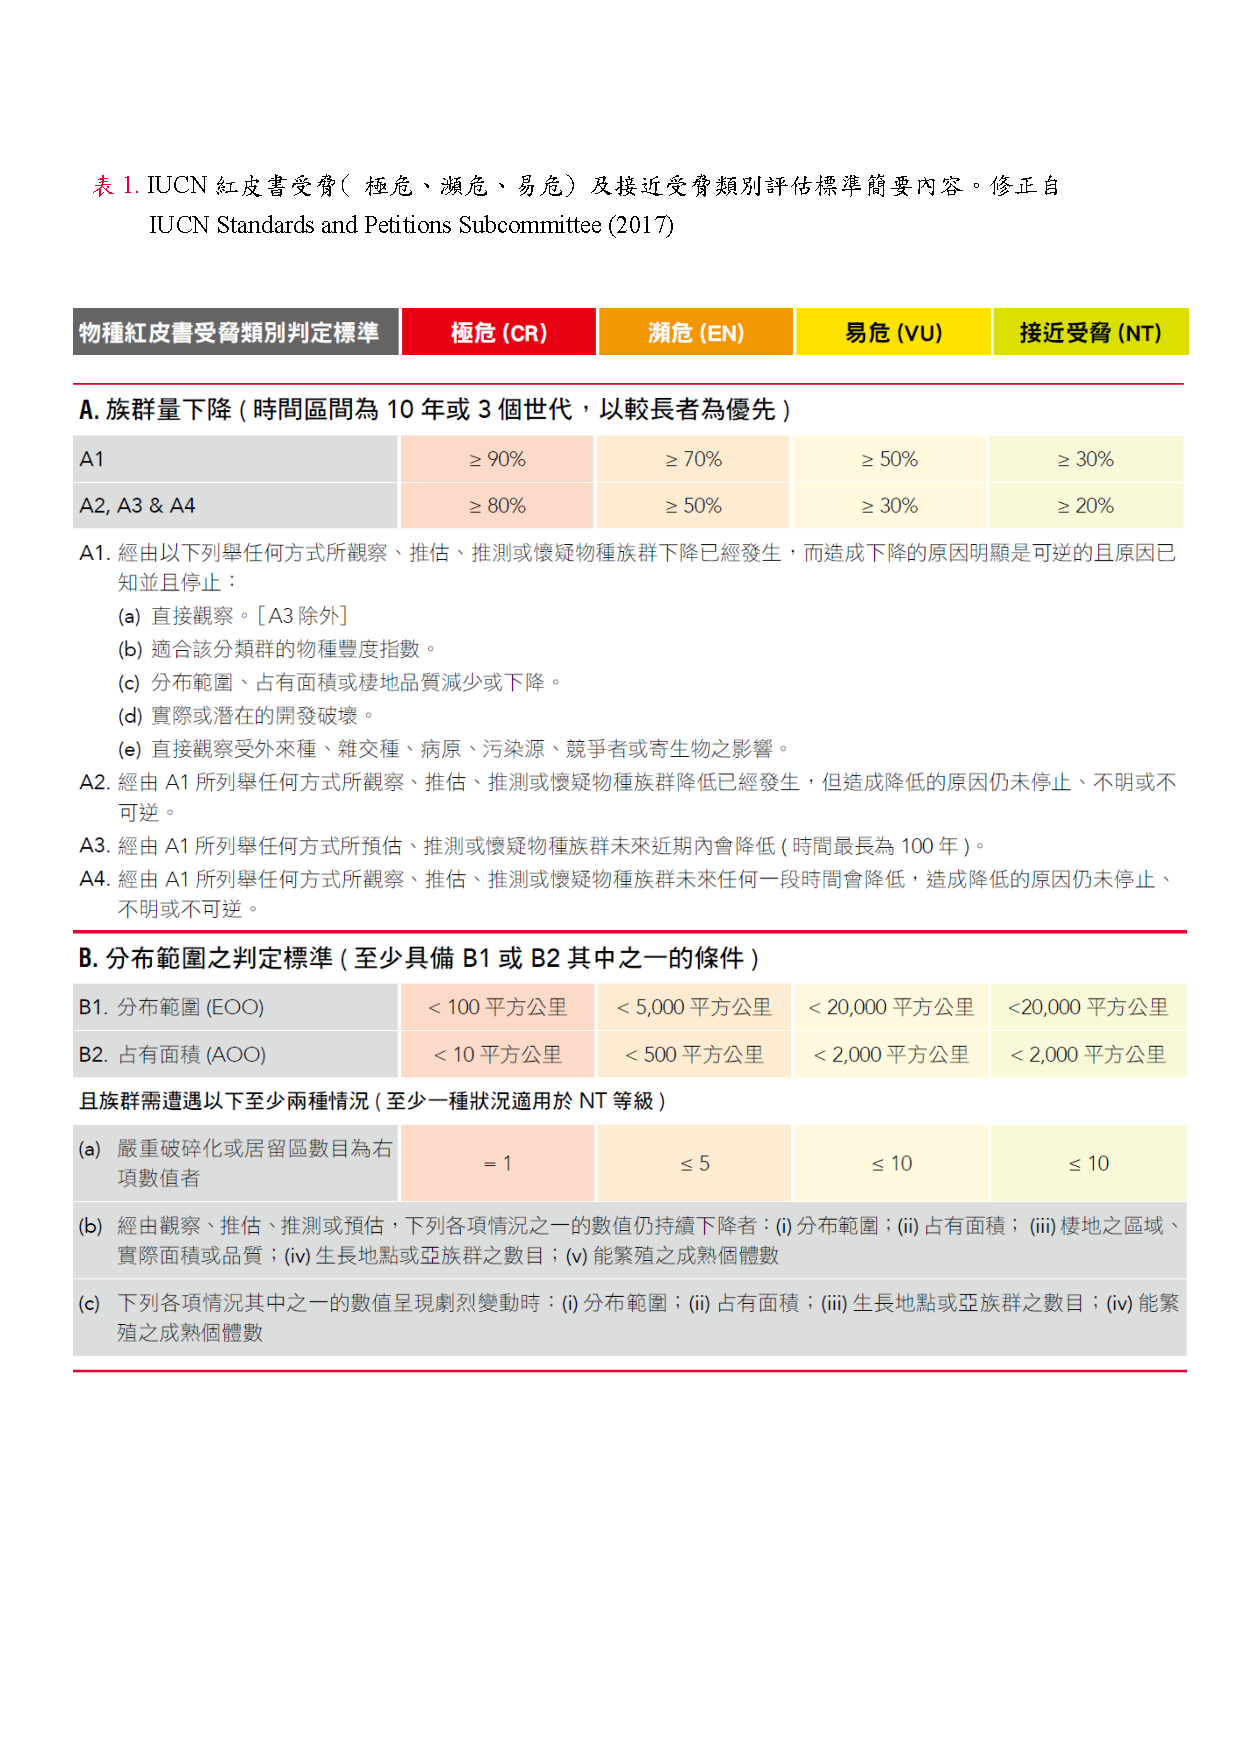
\includepdf{iucn_standards.pdf}
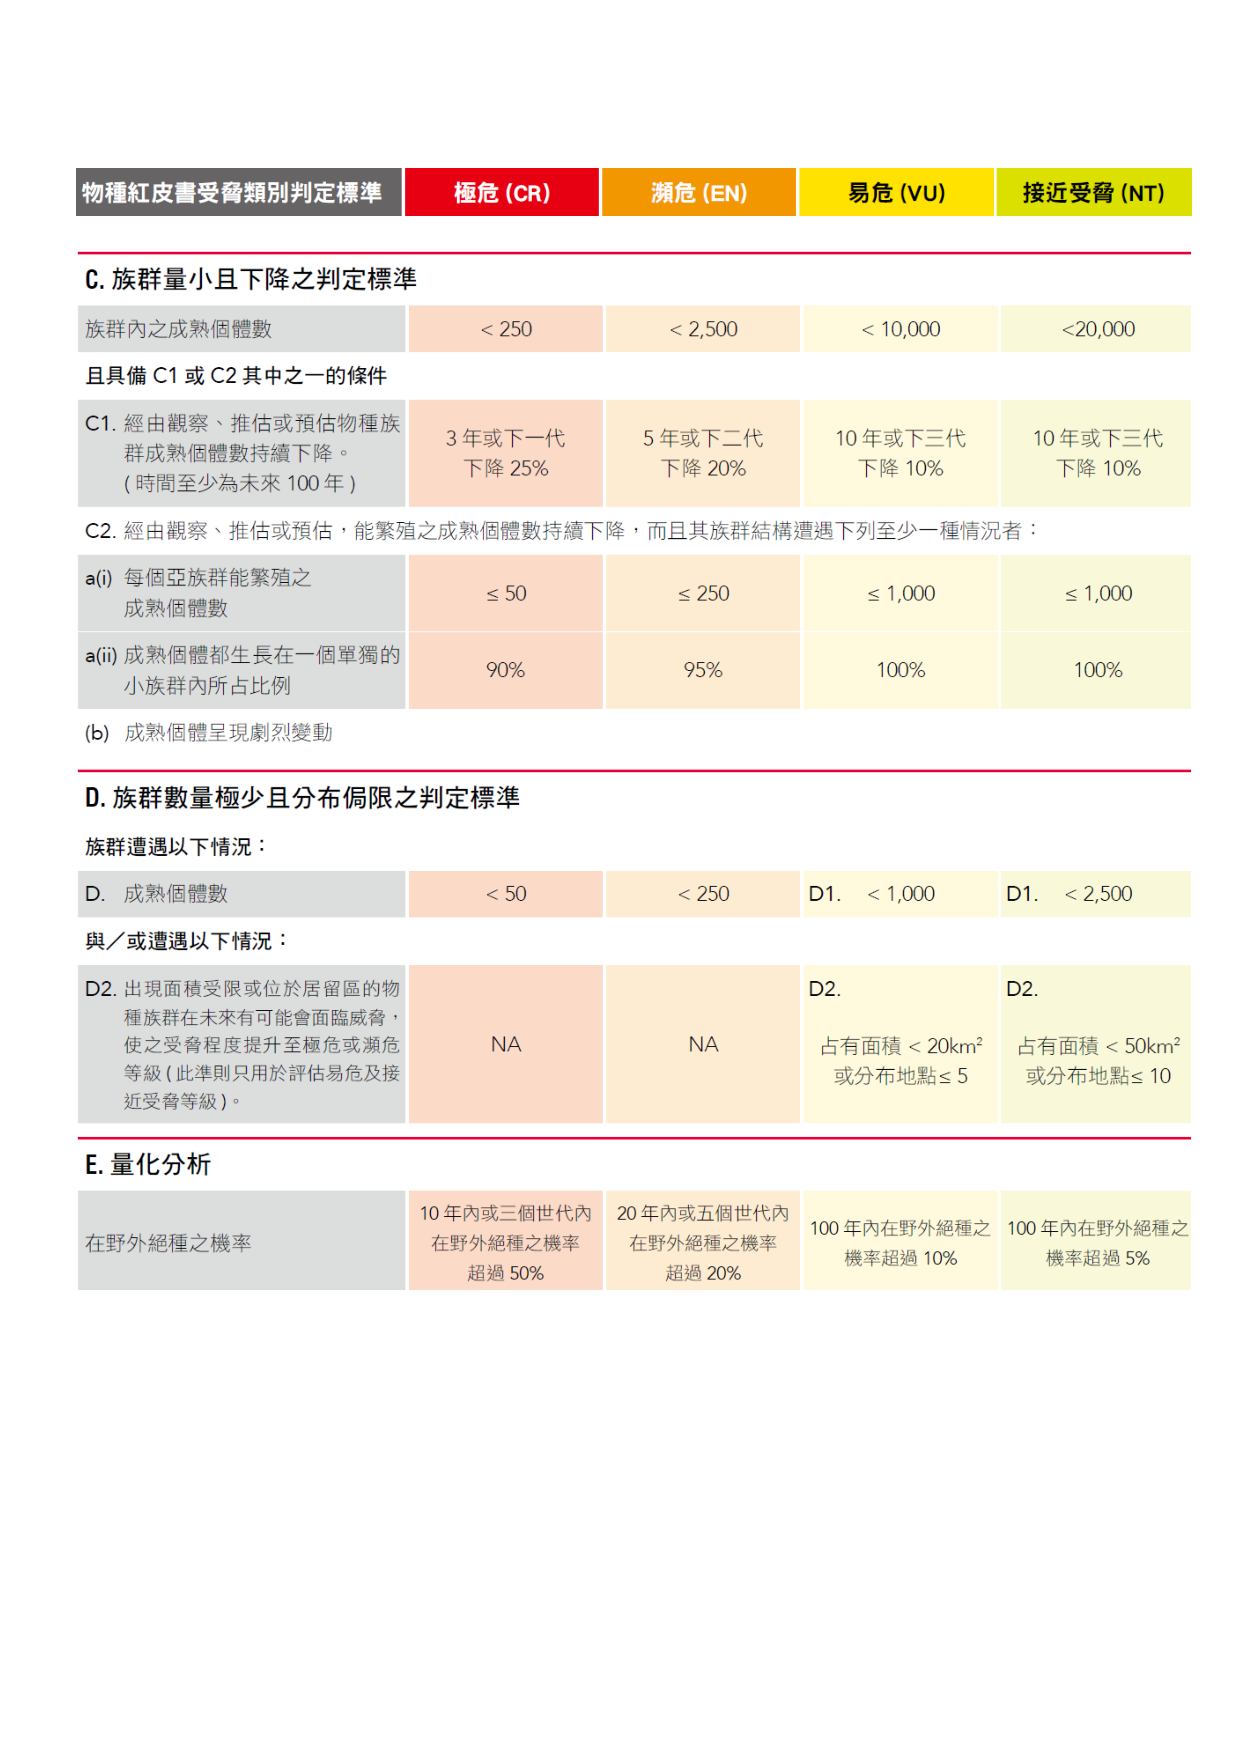
\includepdf{iucn_standards2.pdf}

\section{類別調整}
\begin{multicols}{2}
依據資料完成各分類群的初步類別評估後,如果該分類群非臺灣特有,
需進一步考慮受評估分類群的區域滅絕機率受到評估範圍外相同分類群其他族群的影響程度
(IUCN 2012a) ,
並依據評估結果將該分類群的初步類別予以升級、降級或維持不變。
調整類別的原則依照 IUCN(2012a) 建議流程,針對臺灣族群區域標準,說明如下:


\end{multicols}

\fbox{
    \begin{minipage}{0.9\textwidth}
\begin{enumerate}
    \item[1.] 若該分類群為臺灣特有,維持步驟 2.2 之評估類別結果。 \\
    \item[2.] 若該分類群非臺灣特有,則再依下列原則進行評估,並依據評估結果將該分類群的類別予以升級、降級或維持不變:\\
    \begin{enumerate}
        \item[(1)] 如果原分布地區或臺灣地區的棲息地環境有惡化現象,其類別保持不變。\\
        \item[(2) ] 如果在相鄰地區沒有同種族群或其繁殖體不能播遷到臺灣,臺灣族群可以視為本地特有的,其 類別保持不變。\\
        \item[(3) ] 如果區外族群個體不可能在臺灣存活,類別保持不變。 \\
        \item[(4) ] 如果沒有足夠的適宜棲息地或是現有保護措施不能在可預見的將來改善棲息地環境,區外的移入將不會降低絕滅危險,類別保持不變。\\
        \item[(5) ] 如果分類群在區外相對比較普遍,沒有族群衰退的跡象,且能夠播遷並有(或即將有)可利用的潛在棲息地,則降低其等級。如果分類群在相鄰地區正在減少,「救助影響」不容易發生,則提高類別。\\

        \item[(6) ] 如果有跡象表明一定數量的繁殖體定期到達該地而族群仍然只有少量存活,則地區族群可能爲「數量衰減」。若是如此,繁殖體移入有即將停止的趨勢,提高類別。 \\
    \end{enumerate}
\end{enumerate}
\end{minipage}
}


\section{公開意見徵詢}
\begin{multicols}{2}
經由步驟 2.1 至 2.3 產生的評估結果,於 2017 年 6 月至 11 月徵求並彙整臺灣植物分類 學會全體會員及全國相關機關(如林試所、中研 院生物多樣性中心、自然科學博物館...等)、團 體及個人對於評定類別是否有所不當而需修改
之意見,並於 2017 年 12 月 1 日與林務局共同 召開「臺灣維管束植物紅皮書成果說明會」, 廣泛徵求意見,最後再依據更新之資訊,再次 執行 2.1 至 2.3 步驟後產生本報告。

\end{multicols}
